\documentclass[conference]{IEEEtran} % Use 'journal' for journal articles, 'conference' for conference papers, etc.
\usepackage[utf8]{inputenc}
\usepackage[spanish]{babel}
\usepackage{cite} % For citations
\usepackage{hyperref}
\usepackage{graphicx}

\title{Explorando la Relación entre la Composición de los Elementos y la Superconductividad a Altas Temperaturas mediante Redes Neuronales Densas}
\author{\IEEEauthorblockN{Eber David Gayt\'an Medina}
\IEEEauthorblockA{\textit{Centro de Investigación Científica y de Educación Superior de Ensenada - Introducci\'on a la Ciencia de Datos} \\
eber@cicese.edu.mx}

}

\begin{document}

\maketitle

\begin{abstract}
Your abstract here.
\end{abstract}

\section{Introducción}

El desarrollo de superconductores a temperatura ambiente es uno de los desafíos más 
importantes en la física de materiales. La necesidad de materiales que sean fáciles 
de producir, estables a temperaturas cercanas a las ambientales, y que mantengan sus 
propiedades a lo largo de un rango térmico, es fundamental para diversas aplicaciones 
tecnológicas que podrían transformar sectores clave de la economía global.

Un área de gran impacto es la computación cuántica, donde los superconductores son 
esenciales para la operación de los qubits, unidades básicas de información cuántica. 
Estos dispositivos requieren temperaturas extremadamente bajas para mantener la 
coherencia de los qubits y evitar la pérdida de información cuántica, pero el 
desarrollo de materiales que funcionen a temperatura ambiente podría superar las 
limitaciones actuales y acelerar la adopción de la computación cuántica a gran 
escala \cite{Bassman_Oftelie_2024}.

Por otro lado, los superconductores ofrecen soluciones potenciales para problemas 
críticos en la producción y transporte de energía eléctrica. Actualmente, una 
gran cantidad de energía se pierde durante el transporte debido a la resistencia 
en las líneas de transmisión, lo que genera calor y reduce la eficiencia energética~\cite{sarajcev2000calculation}. 
Los superconductores eliminan esta resistencia, permitiendo la transmisión de energía 
sin pérdidas y mejorando la eficiencia de las redes eléctricas, lo cual podría ser
revolucionario para la industria energética global.

Además, los superconductores tienen aplicaciones en trenes de levitación magnética, 
dispositivos de almacenamiento de energía como los sistemas de almacenamiento de energía magnética por
superconducción (SMES) que almacenan energía de la misma forma que
lo haría un inductor convencional, con la principal diferencia de que
la corriente directa fluye a través de un alambre superconductor significando
que el alambre se encuentra a temperaturas criogénicas
y no muestra resistencia conductiva alguna~\cite{gonzalez2013almacenamiento}. Otros ejemplos son en la 
diagnosis médica (para imágenes de resonancia magnética), centros de
investigación (equipos de resonancia magnética nuclear, aceleradores, reactores de fusión) y
procesos industriales (separación magnética), donde la eficiencia y el control de los 
campos magnéticos son esenciales.

\subsection{Objetivo}
Dada la relevancia de estos avances, las investigaciones sobre nuevos materiales 
superconductores ya no solo son valiosas, sino necesarias. Para acelerar el 
descubrimiento de nuevos materiales con estas propiedades, el uso de herramientas 
avanzadas como el aprendizaje automático se vuelve crucial, permitiendo predecir 
y validar compuestos prometedores antes de su fabricación y prueba experimental~\cite{coll2017superconductividad}.

\section{Metodología}
Se utilizaron dos~\href{https://www.kaggle.com/datasets/tunguz/superconductivty-data-data-set/code}{Datasets}, 
el primero se hizo a partir un conjunto de datos con descriptores químicos y 
físicos de materiales, con el objetivo de establecer una relación entre la 
composición de los elementos y la superconductividad a altas 
temperaturas. El segundo es la base y tiene el formato de material y temperatura critica.
Para asegurarse de condensar la mayor cantidad de información en un solo data set ase hizo 
un ``merge'' a partir de la temperatura critica, uniendo 82 columnas
del primer dataset y 87 del segundo.
 
\subsection{Conjunto de datos}
El conjunto de datos empleado consta de 168 atributos que describen la 
composición y las propiedades de los materiales superconductores, con 
temperaturas críticas que oscilan entre 0 y 140 K. Los atributos se 
generaron a partir de análisis químicos, físicos y estadísticas 
descriptivas de los elementos que componen cada material.

\subsection{Preprocesamiento}

\subsection{Gestión de Datos Desbalanceados} Se exploró la distribución de 
las temperaturas críticas para identificar posibles desbalances. 
Se emplearon histogramas y gráficos de densidad para visualizar 
la distribución.

\subsubsection{Estandarizacion}
Se obtuvo que los datos estaban desvalanceados hacia temperaturas 
cercanas al 0 absoluto, por lo tanto se hizo una transformación 
z-score para de modo que todos los atributos contribuyan de manera 
equitativa al entrenamiento del modelo, evitando que los atributos 
con mayores magnitudes dominen el proceso.

\subsubsection{División del Conjunto de Datos}
El conjunto de datos fue dividido 
en un conjunto de entrenamiento (80\%) y un conjunto de prueba 
(20\%) de manera aleatoria, asegurando que las propiedades 
estadísticas de la distribución se mantuvieran.

\subsection{Arquitectura del Modelo}

Se diseñó un modelo de red neuronal profunda utilizando Keras, se usaron 
capas densas con la justificación de atacar una problemática con muchos 
atributos. Al con 
la siguiente arquitectura:
\begin{itemize}
    \item Una capa densa de 256 neuronas con función de activación ReLU, 
    seguida de una capa de Dropout (0.3) para prevenir el sobreajuste.
    \item Una segunda capa densa de 128 neuronas con ReLU, seguida de una 
    capa de Dropout (0.3).
    \item Capas adicionales de 64, 32 y 16 neuronas con ReLU para capturar
    características complejas.
    \item Una capa de salida de 1 neurona sin función de activación, adecuada 
    para un problema de regresión.
\end{itemize}

El modelo fue compilado con el optimizador Adam y una tasa de 
aprendizaje inicial de 0.001, utilizando el error cuadrático medio 
(MSE) como función de pérdida y el error absoluto medio (MAE) como 
métrica de evaluación.

\subsection{Entrenamiento}

Se entrenó el modelo durante 25 épocas con un tamaño de lote de 32 
muestras. Se implementó un programador de tasa de aprendizaje que 
redujo la tasa a la mitad cada 10 épocas para optimizar la 
convergencia. Además, se usaron conjuntos de datos de validación 
para monitorear el rendimiento y ajustar los hiperparámetros.

\subsection{Evaluación}

El rendimiento del modelo se evaluó utilizando el MAE, el RMSE y 
el coeficiente de determinación $(R^2)$ en el conjunto de prueba. 
Además, se compararon los resultados con modelos de referencia, 
como Random Forests y métodos de regresión tradicionales, 
reportados en estudios previos. Se generaron gráficos de dispersión 
para analizar visualmente las predicciones frente a los valores 
reales de temperatura crítica.

\section{Resultados}

En esta sección, se presentan los resultados obtenidos al aplicar 
el modelo de red neuronal profunda para predecir la temperatura 
crítica de los materiales superconductores. Se analizan las 
métricas de rendimiento, visualizaciones clave y la importancia 
de los atributos.

\subsection{Desempeño del Modelo}

Usando el modelo propuesto, se hicieron las predicciones
del apartado de prueba. El resultado, como se puede observar en
la figura~\ref{fig:Entrenamiento} es fácil apreciar que en su mayoría,
las predicciones de temperatura crítica fueron acertadas.

\begin{figure}[!h]
    \centering
    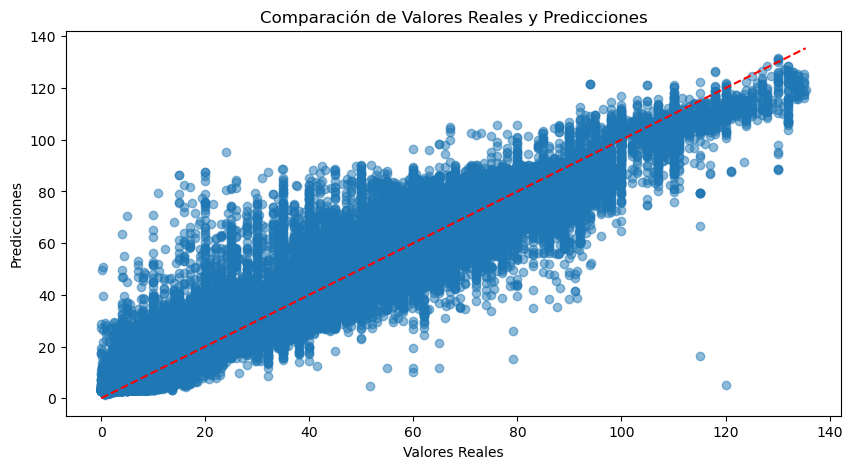
\includegraphics[width=0.5\textwidth]{Entrenamiento.png}
    \caption{Gráfico de dispersión de las temperaturas reales enfrentados contra las temperaturas predichas.}
    \label{fig:Entrenamiento}
\end{figure}

Se uso MSE, $R^2$, RMSE y MAE para hacer las validaciones, dando como resultado:
$$RMSE: 6.4965$$
$$R^2 Train: 0.9621$$
$$R^2 Test: 0.9592$$





\section{Discusión y conclusiones}

Falta un análisis de la composición de cada 
Conclude your paper.

\bibliographystyle{ieeetr} % Use the IEEEtran bibliography style
\bibliography{bibliografia.bib} % Replace with your .bib file name

\end{document}
